% Condensed results section: F1, F2, F3 findings with headline numbers and figures
% Data: sections/results.tex (long-form), findings.md (F1-F3 empirical summaries)
% Target: ~2.5 pages; defer detail to Appendix~\ref{app:repro}, Appendix~\ref{app:training}

This section reports three empirically grounded findings from pretraining on the BabyLM budget. Finding 1 (F1) characterizes the scale-dependent effect of dropping the auxiliary causal language modeling (CLM) head in favor of pure masked-language modeling (MLM) pretraining. Finding 2 (F2) evaluates kāraka role-stratified masking as a causal mechanism at matched budget. Finding 3 (F3) assesses a supervised kāraka-role auxiliary objective across 5 pre-registered seeds. Collectively, these findings show that robust gains arise from architectural choices such as rotary position embeddings (RoPE) and the choice of pretraining objective (pure MLM at scale), while Pāṇinian mechanisms contribute design clarity and interpretability without validated improvements to BLiMP performance. Table~\ref{tab:headline} first situates both submission tracks against their own official baseline.

\begin{table}[t]
\centering
\caption{Both submission tracks against their own official BabyLM baseline~\cite{Hu2024BabyLM}.}
\label{tab:headline}
{\small
\begin{tabular}{llcccc}
\toprule
Track & Model & Budget & BLiMP & Official baseline & $\Delta$ \\
\midrule
Strict & prabhasa-b\_s & 100M & 73.06 \,(n\,=\,1) & 74.53 & $-1.47$ \\
Strict-Small & prabhasa-b\_ss-0.1 & 10M & 64.09 \,($\pm$0.26) & 65.08 & $-0.99$ \\
\bottomrule
\end{tabular}
}
\end{table}

\subsection{F1: Scale-Dependent Objective Effect}

The auxiliary CLM head, which predicts the previous token given future context, may dilute the MLM training signal at scale. Pure-MLM and hybrid models are trained identically except for the objective, using three independent seeds at 10M (Strict-Small baseline 65.08) and single seeds at 100M (Strict baseline 74.53). At 10M, pure-MLM achieves a 3-seed mean of 63.58 (95\% CI \(\pm\) 1.73), while hybrid yields 64.09 (95\% CI \(\pm\) 0.26); confidence intervals overlap, indicating no significant difference. At 100M (n\,=\,1 per variant), pure-MLM achieves 73.06 BLiMP versus hybrid at 67.57 BLiMP, a 5.49 percentage point advantage. Figure~\ref{fig:objscale} visualizes this scale-dependent divergence: the gap widens from neutral at 10M to 5.49 pp at 100M. The regularizing effect of the CLM head at 10M becomes a capacity bottleneck to MLM signal quality at larger scales. The 10M neutral result justifies retaining hybrid for the Strict-Small submission (prabhasa-b\_ss-0.1), while the single-seed 100M pure-MLM result drives the Strict-track model design.

\begin{figure}[h]\centering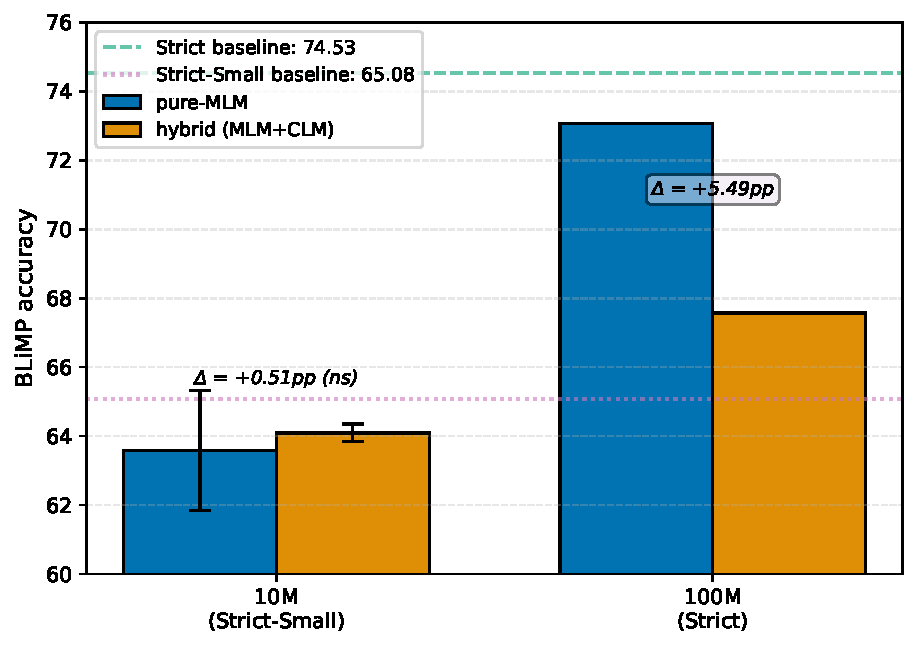
\includegraphics[width=0.58\linewidth]{figures/fig_objective_scale.pdf}
\caption{F1 scale-dependent objective effect: pure-MLM versus hybrid MLM\texttt{+}CLM across 10M and 100M.}
\label{fig:objscale}\end{figure}

\subsection{Strict-Track Results: prabhasa-b\_s (100M, Pure-MLM)}

The 100M pure-MLM model (prabhasa-b\_s, n\,=\,1) is evaluated on the full official BabyLM Strict-track test suite. The Strict-track baseline achieves 74.53 BLiMP~\cite{Hu2024BabyLM}. The model underperforms on main BLiMP by 1.47 percentage points (73.06 versus 74.53) but gains 2.46 percentage points on BLiMP Supplement (67.46 versus 65.0) and 9.66 percentage points on Entity Tracking (33.26 versus 23.6). The Text Average of 55.99 exceeds the baseline reference of 54.0, suggesting competitive overall generalization despite the main-BLiMP shortfall. Detailed per-category results appear in Appendix~\ref{app:repro}.

\subsection{F2: Kāraka-Masking Causality (Matched-Budget Comparison)}

Kāraka role-stratified masking (Arm K) is compared to uniform-random masking (Arm C) at identical mask budget (100M, n\,=\,1 per arm). The experimental configuration is held constant: N-hot morpheme embeddings, RoPE, pure-MLM objective, identical frequency weighting. Per pre-registration (cycle 21), the primary metric is paired bootstrap over 20 targeted paradigms (agreement and argument-structure tasks). Arm K achieves 71.77 full BLiMP, Arm C achieves 70.49. On the targeted subset, Arm K scores 82.03 and Arm C scores 81.93. The paired bootstrap yields \(\Delta_{K-C} = +0.10\) percentage points (95\% CI [−0.99, +1.20]), not significant. Figure~\ref{fig:f2_karaka} visualizes this null effect of role-stratification at matched budget. Earlier exploratory runs reported +1.23 pp gains from kāraka masking, but those reflected confounds (higher mask rates, frequency-weighting) not budget-matched. With matching enforced, role-stratified distribution contributes no signal. F2 is a pre-registered null; additional interventions (real deprel parses, 3-seed replication) are queued.

\begin{figure}[h]\centering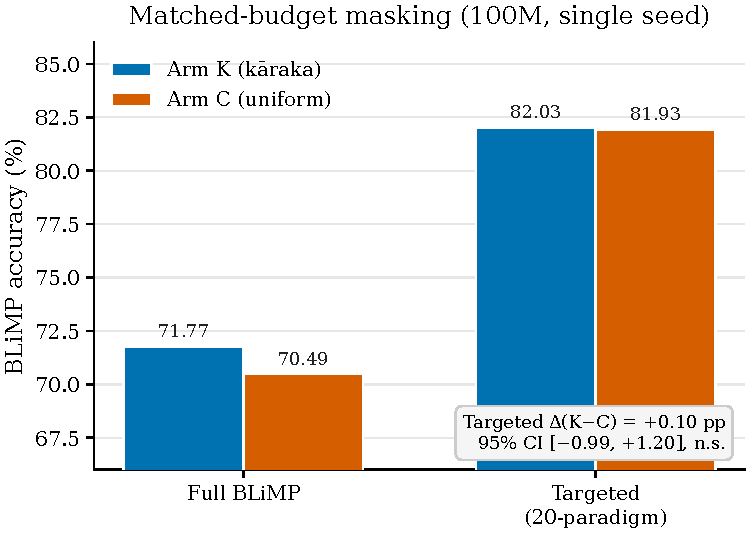
\includegraphics[width=0.58\linewidth]{figures/fig_f2_karaka.pdf}
\caption{F2 kāraka masking causality: Arm K versus Arm C on targeted subset (100M).}
\label{fig:f2_karaka}\end{figure}

\subsection{F3: Kāraka Auxiliary Objective (5-Seed Paired t-Test)}

The supervised kāraka-role prediction auxiliary objective is a token-level multi-task head trained to predict roles from the MLM hidden state (10M, n\,=\,5). The objective weight is \(\lambda = 1.0\) for auxiliary and \(\lambda = 0.0\) for baseline; corpus, masking, and seed list are held fixed. Per pre-registration (cycle 6, extended cycle 60), the primary metric is the per-seed targeted-subset delta (\(\Delta_{\text{aux}-\text{base}}\)) on 20 paradigms, tested via paired t-test. The 5-seed targeted mean yields auxiliary 74.02 versus baseline 73.26 (+0.76 pp, 95\% CI [−0.74, +2.27]; t = 1.41, df = 4, not significant). The effect attenuates with sample size: +2.65 pp at 1 seed, +1.46 pp at 3 seeds, +0.76 pp at 5 seeds, indicating the initial result reflected seed luck. Figure~\ref{fig:f3} displays the per-seed delta distribution and attenuation; full per-seed scores appear in Appendix~\ref{app:repro}. A specificity control tests whether improvement is kāraka-specific or generic multi-task regularization: real-auxiliary (74.41, 3-seed mean) exceeds shuffled-role (73.53) and baseline (72.95), and shuffled-role does not recover the real effect, ruling out generic regularization though all contrasts are wide and not significant. F3 is classified weak non-significant: a consistent positive direction resisting shuffled-role control suggests kāraka-specificity, but the effect is underpowered at 10M. The 74-paradigm BLiMP results parallel targeted findings (real-auxiliary 64.89 versus baseline 63.88, +1.01 pp, ns).

\begin{figure}[h]\centering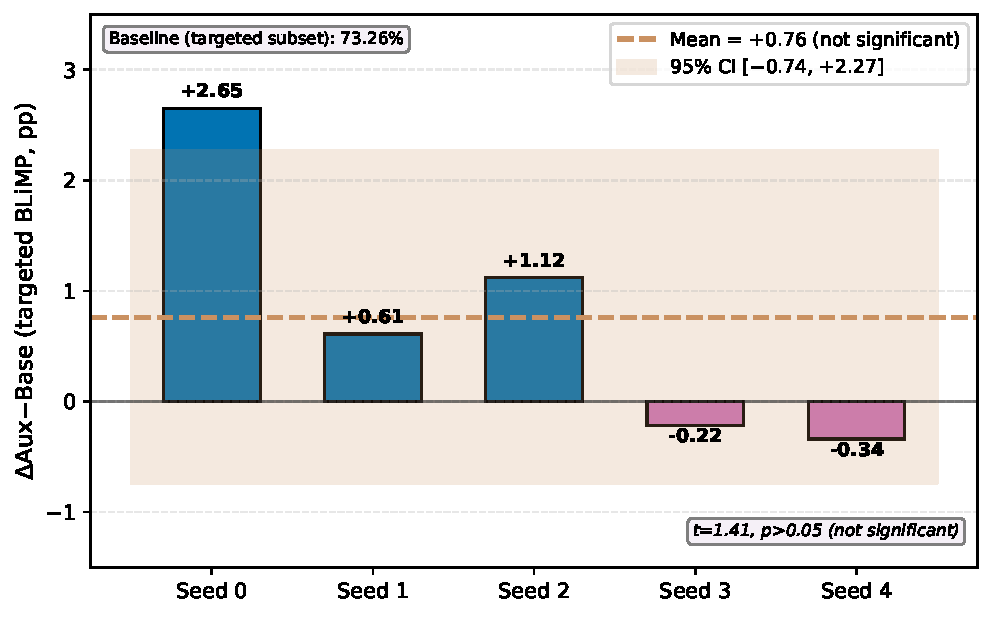
\includegraphics[width=0.58\linewidth]{figures/fig_f3_seeds.pdf}
\caption{F3 auxiliary objective: per-seed delta across 5 seeds on targeted subset (10M).}
\label{fig:f3}\end{figure}

\subsection{Strict-Small Track and GLUE Fine-Tuning}

The 10M model (prabhasa-b\_ss-0.1, n\,=\,3) is evaluated on the BabyLM Strict-Small track (baseline 65.08 BLiMP). Three seeds yield individual BLiMP scores 65.22, 63.31, and 62.20, with 3-seed mean 64.09 (95\% CI \(\pm\) 0.26), slightly below baseline but within confidence interval, indicating competitive performance. Following pretraining, the model is fine-tuned on 7 GLUE tasks (BoolQ, MultiRC, RTE, WSC, MRPC, QQP, MNLI). Macro-average GLUE score is 0.581 (58.1\%), with strongest results on WSC (0.673 accuracy) and MRPC (0.813 F1), and lowest on MNLI (0.342 accuracy). The model recovers on binary and structured-matching tasks but struggles with complex multi-class inference, consistent with the 10M pretraining budget. Detailed per-seed BLiMP and task-by-task GLUE results appear in Appendix~\ref{app:repro}.

Taken together, the three findings localize the robust gains to the RoPE architecture and the pure-MLM objective at scale, while the Pāṇinian mechanisms contribute role-based linguistic structure and design clarity without a validated improvement in BLiMP performance. Section~\ref{sec:discussion} interprets these outcomes and their implications.
